\documentclass[11pt]{beamer}
\usetheme{simple}
\setbeamertemplate{footline}{} 
\usepackage{tikz}
\usepackage{pgfplots}
\usepackage{amsmath, amssymb, amsthm}   
\pgfplotsset{
        % declare the function you want to plot so you can reuse it easily later
        /pgf/declare function={
            T1(\u)=ln(0.5*(-2*\u+sqrt(4+4*\u^2)));
            T0(\u)=ln(0.5*(2*\u+sqrt(44+4*\u^2)));     
            U0(\u)=\u-1;
            T12(\u)=ln(-1-2*\u);
        },
        % define style to use for the plot to draw only ticks at `\myxlist'
        % (the plot should be invisible)
        my ticks/.style={
            samples at={\myxlist},
            mark=none,
            draw=none,
%            only marks,     % <-- uncomment me to show the data points
        },
every non boxed y axis/.append style={y axis line style=-}
    }
%\pgfplotsset{ every non boxed y axis/.append style={y axis line style=-}}
\setbeamertemplate{navigation symbols}{}
\begin{document}
\begin{frame}


\tikzset{every picture/.style={line width=0.75pt}} %set default line width to 0.75pt        

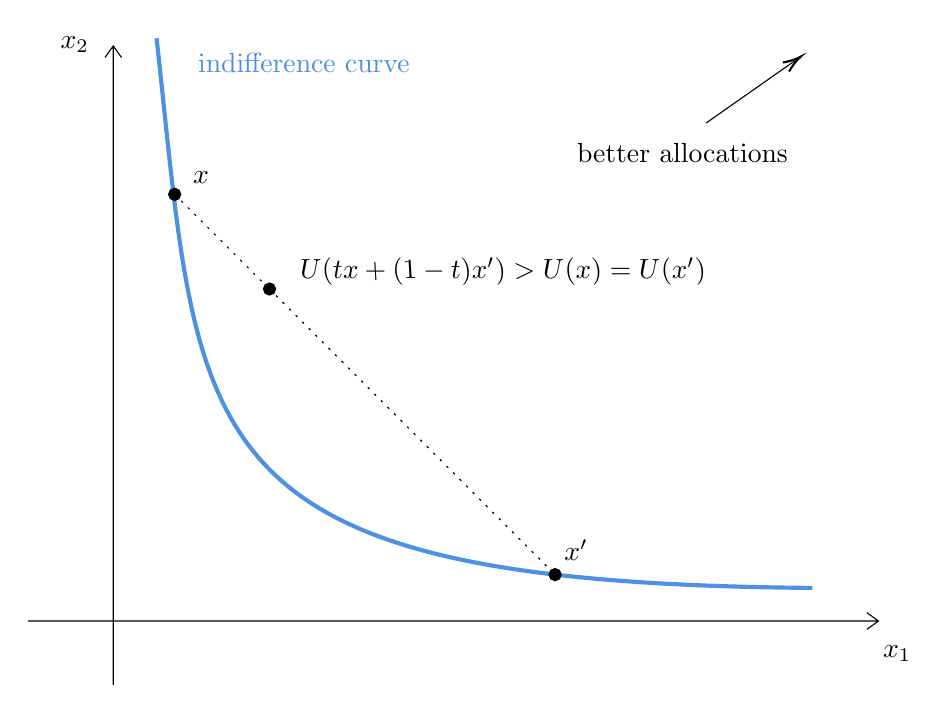
\begin{tikzpicture}[x=0.75pt,y=0.75pt,yscale=-.8,xscale=.8]
%uncomment if require: \path (0,443); %set diagram left start at 0, and has height of 443

%Shape: Axis 2D [id:dp11877989343343409] 
\draw  (74,382.93) -- (586.09,382.93)(125.21,36.6) -- (125.21,421.41) (579.09,377.93) -- (586.09,382.93) -- (579.09,387.93) (120.21,43.6) -- (125.21,36.6) -- (130.21,43.6)  ;
%Curve Lines [id:da6451900492142217] 
\draw [color={rgb, 255:red, 74; green, 144; blue, 226 }  ,draw opacity=0.99 ][line width=1.5]    (151.3,32) .. controls (178.3,276) and (164.3,360) .. (546.3,363) ;


%Straight Lines [id:da3745755779223563] 
\draw  [dash pattern={on 0.84pt off 2.51pt}]  (219.3,183) -- (391.3,355) ;
\draw [shift={(391.3,355)}, rotate = 45] [color={rgb, 255:red, 0; green, 0; blue, 0 }  ][fill={rgb, 255:red, 0; green, 0; blue, 0 }  ][line width=0.75]      (0, 0) circle [x radius= 3.35, y radius= 3.35]   ;
\draw [shift={(219.3,183)}, rotate = 45] [color={rgb, 255:red, 0; green, 0; blue, 0 }  ][fill={rgb, 255:red, 0; green, 0; blue, 0 }  ][line width=0.75]      (0, 0) circle [x radius= 3.35, y radius= 3.35]   ;
%Straight Lines [id:da43649223131894366] 
\draw  [dash pattern={on 0.84pt off 2.51pt}]  (162.2,126) -- (219.3,183.1) ;

\draw [shift={(162.2,126)}, rotate = 45] [color={rgb, 255:red, 0; green, 0; blue, 0 }  ][fill={rgb, 255:red, 0; green, 0; blue, 0 }  ][line width=0.75]      (0, 0) circle [x radius= 3.35, y radius= 3.35]   ;
%Straight Lines [id:da2746283553273896] 
\draw    (482.3,83) -- (537.66,44.15) ;
\draw [shift={(539.3,43)}, rotate = 504.94] [color={rgb, 255:red, 0; green, 0; blue, 0 }  ][line width=0.75]    (10.93,-3.29) .. controls (6.95,-1.4) and (3.31,-0.3) .. (0,0) .. controls (3.31,0.3) and (6.95,1.4) .. (10.93,3.29)   ;


% Text Node
\draw (597.35,402.33) node   {$x_{1}$};
% Text Node
\draw (360,172.6) node [xslant=-0.06]  {$U( tx+( 1-t) x')  >U( x) =U( x')$};
% Text Node
\draw (178,116) node   {$x$};
% Text Node
\draw (404,340) node   {$x'$};
% Text Node
\draw (102,36) node   {$x_{2}$};
% Text Node
\draw (240,47) node [color={rgb, 255:red, 74; green, 144; blue, 226 }  ,opacity=1 ] [align=left] {indifference curve};
% Text Node
\draw (468,101) node  [align=left] {better allocations};


\end{tikzpicture}
\end{frame}
\end{document}